\section{FWHM change on piezo position}
Using the dual-piezo setup, we decided to analyze the hysteresis of the piezo. To do this, the scan was once again actiaveted with the following setting:
\subsubsection*{Scan-Settings}
$f = 6.0$ Hz,  \\
Amplitude: 5.2 V,  \\
Offset: 0 V.  \\
Piezo No.; \texttt{2}  \\
Script: \texttt{analyzeFWHMvsPiezo.m} \\

The second piezo was used to change the position of the peaks using a DC offset voltage.
I changed to position of an arbitrary large Peak from the left most side of the scan to the right most side of the scan. I recorded the transmission signal for dozens of piezo offset voltages in order to see a change. Ideally, the relative position of the peak compared to the scan should not matter, but as seen previously, it does. 


\begin{figure}[H]
    \centering
    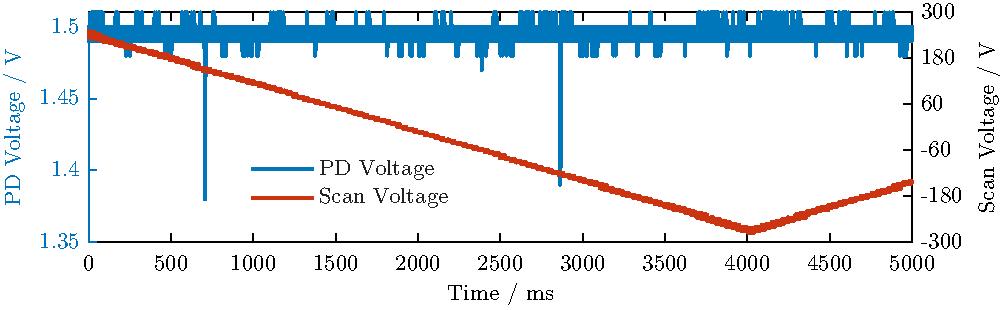
\includegraphics[width=\textwidth]{fwhm/Figure_1.pdf}
    \caption{Example frame, where the peak investigated is still fairly to the left of the scan. The x axis has been cut-off to represent only the length of one direction of a scan (here roughly from 58 to 143 ms). The position of main peak is marked in black (this does not indicate the fitting, only the position on the x axis) and a second peak has been marked in pink, which will also be used for analysis.}
\end{figure}


\begin{figure}[H]
    \centering
    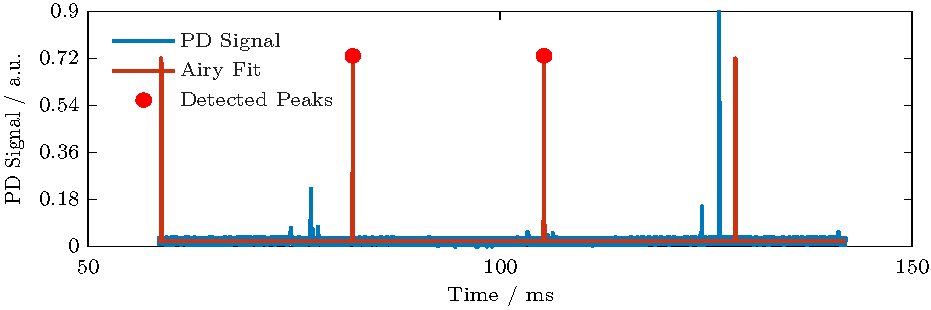
\includegraphics[width=\textwidth]{fwhm/Figure_2.pdf}
    \caption{Now, the two peaks have moved to the right side of the scan. Clearly, the time distance between the peaks has gotten shorter. Also, if you look at the title, the FWHM has also shrunk.}
\end{figure}

The FWHM have been determined by a Lorentzian Fit around the peak. I made sure to always analyze the same peak. Combining dozens of offset voltages, we get the following plots showing the FWHM deviation as well as the spacing between the two adjacend peaks. The x axes have been scaled to show the voltage of the scanned piezo at the position of the peak


\begin{figure}[H]
    \centering
    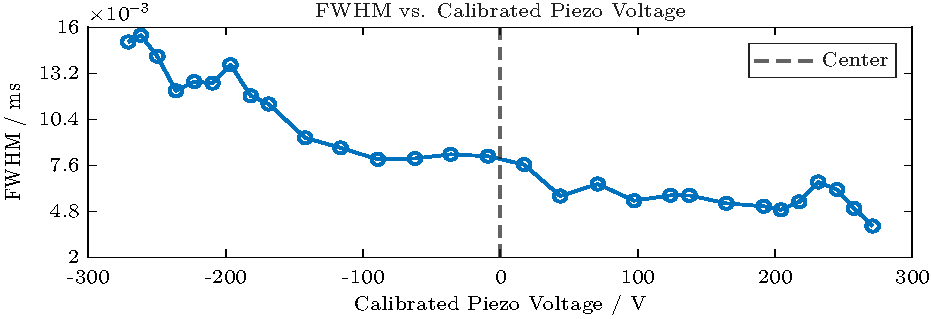
\includegraphics[width=\textwidth]{fwhm/Figure_3.pdf}
    \caption{This plot shows the change in FWHM coming from one side of the scan the other. It is clear that the FWHM did change significantly (by a factor of around 3.8). The x axis represents the voltage of the scanning piezo for each peak position.}
\end{figure}


\begin{figure}[H]
    \centering
    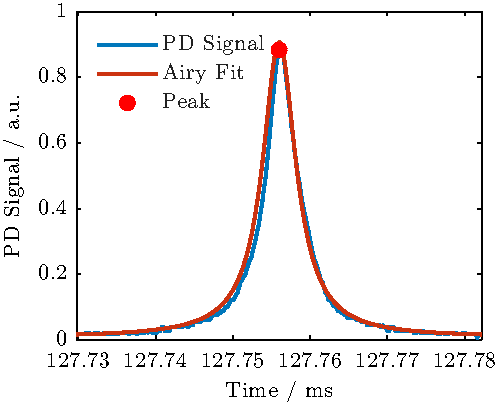
\includegraphics[width=\textwidth]{fwhm/Figure_4.pdf}
    \caption{Once again, the distance between the two adjacend peaks differs significantly from one side to the other with a factor of 3.2 (this cant be directly compared to the previous factor, as the adjacent peak was not captured in the first couple of measurements. If we compare the range where both the FWHM and the peak distances has been captured, this factor is nearly identical)}
\end{figure}

Unfortuneatley, it seems that during the run of this measurements, the piezo that was used with a DC offset voltage has been damaged. 
